\chapter{Pruning}\label{ch:pruning}
In \autoref{ch:introduction} I gave a brief explanation of few techniques for
doing model optimisation on a neural network. Pruning is one of these and in
the first part of this chapter I give a more detailed explanation.
The second part instead focuses on the core of the thesis: per-layer pruning
configuration with heuristic.

Despite being technical, this chapter is still fairly theoretical and I defer
any code and implementation to \autoref{ch:implementation}.

\section{What's Pruning?}
Neural network pruning is the task of reducing the size of a network by
removing parameters. This compression affects the size of the model, the
latency, the amount of memory and the compute power needed to run the
inference. These metrics need to balanced with the accuracy of the model
itself. I give a more detailed analysis about this trade-off in
\autoref{subsec:tradeoff}

Pruning has been used since the late 1980s but has seen an explosion of
interest in the past decade thanks to the rise of deep neural networks.
It sets its roots with a couple of classic papers:\textit{Optimal Brain
Damage}~\cite{lecun-90b} and \textit{Optimal Brain Surgeon}\cite{hassibi-93}

In the last decade (2010\-2020) a few dozens of papers have been published in
literature about pruning and all of them have been showing that pruning is an
effective technique that can be applied to a variety of neural network on
different fields (image and speech recognition, text processing, etc\ldots).
Moreover they highlights that pruning is a versatile technique as, I said
earlier, it has a positive impact on multiple metrics, all important for a
better edge deployment of the model.

How does pruning reduce the size of a model? The basic principle is to prune
(remove) unnecessary neurones or weights (see \autoref{fig:pruning_weights_neurons}):

\begin{figure}[ht]
    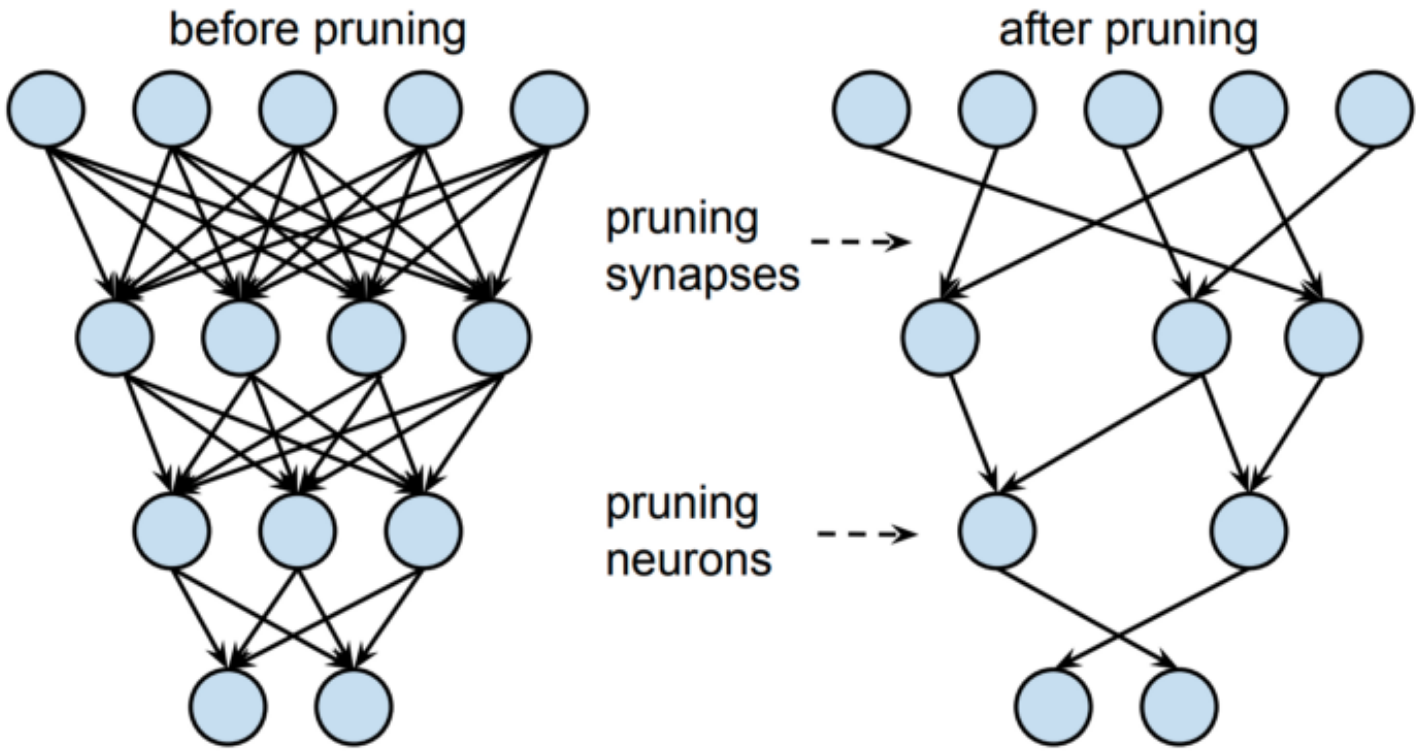
\includegraphics[width=8cm]{images/pruning/pruning_weights_neurons.png}
    \centering
    \caption{Pruning weights and neurons}\label{fig:pruning_weights_neurons}
\end{figure}

\begin{itemize}
    \item \textbf{weights}: this is done by setting individual parameters to
        zero and making the network sparse. The effect will be to maintain the
        same architecture of the network but lowering down the number of
        parameters.
    \item \textbf{neurons}: this is done by removing the entire node from the
        network with all its connections. This would make the network
        architecture smaller but with the target to keep the accuracy of the
        starting network.
\end{itemize}

\subsection{Pruning techniques}
The main problem in pruning is to understand what to prune. Of course the goal
is to remove nodes and/or weights that are less useful. There are different
methods to understand what to prune with very little or no effect on accuracy.
Below e brief description of different techniques.

\subsubsection{Magnitude Pruning}
Functions can be a very simple case of a neural network. Its coefficients can
be changed in order to learn the input data points. There are coefficients
that, despite changing their values, they won't change the behaviour of the
function and these are referred as \textbf{non-significant}.
In neural networks these coefficients are weights and biases: they are
\textbf{trainable parameters} and the same non-significant concept can be
applied to them with bit more complexity.

During the back-propagation (gradient descent) some weights are updated with
larger gradient magnitudes (both positive and negative) than the others.
These weights are the \textbf{significant} ones and the weights receiving very
small gradients can be considered as \textbf{non-significant} as their impact
is minimal to the optimization of the loss function.
After the training, the weight magnitude of every layer can be explored and
check which weights are significant.

So the weight magnitude is the criteria for pruning the neural network.
At this point a \textbf{threshold} is specified and all the weights below this
threshold are considered non-significant. This is usually combined with a
\textbf{sparsity target} the network should achieve.
The \textbf{non-significant weights will be zeroed}, cancelling effectively
their impact in the neural network.
This can be applied to biases as well (to any trainable parameter to be
precise).

Once the pruning is done it's always advisable to retrain the network in order
to compensate for any drop in performance. It's worth noticing that during the
retraining the pruned weights won't be updated.~\cite{magnitude_pruning}

Magnitude pruning is the technique I will be using in
\autoref{ch:implementation}.

\subsubsection{Channel Pruning}
Channel pruning is a technique specifically for CNN (Convolutional Neural
Network) as it rely on the architecture of this type of networks. The building
blocks of a CNN are (see \autoref{fig:cnn}):

\begin{figure}[ht]
    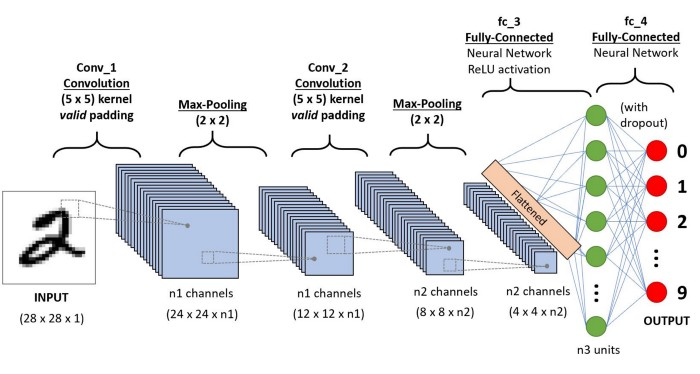
\includegraphics[width=\textwidth]{images/pruning/cnn.jpeg}
    \centering
    \caption{Convolutional Neural Network Architecture}\label{fig:cnn}
\end{figure}

\begin{itemize}
    \item \textbf{Convolutional layer}: it is the core building block of a CNN\@.
        A convolution is the simple application of a filter to an input that
        results in an activation. Repeated application of the same filter to an
        input results in a map of activations called a feature map, indicating
        the locations and strength of a detected feature in an input, such as
        an image.
    \item \textbf{Pooling layer}: it provide an approach to down sampling
        feature maps by summarizing the presence of features in patches of the
        feature map. Two common pooling methods are average pooling and max
        pooling that summarize the average presence of a feature and the most
        activated presence of a feature respectively.
    \item \textbf{ReLU layer}: ReLU stands for \textbf{Rectified Linear Unit}
        and it is a piecewise linear function that will output the input
        directly if it is positive, otherwise, it will output zero. It has
        become the default activation function for many types of neural
        networks because a model that uses it is easier to train and often
        achieves better performance (see \autoref{fig:relu})
\begin{figure}[ht]
    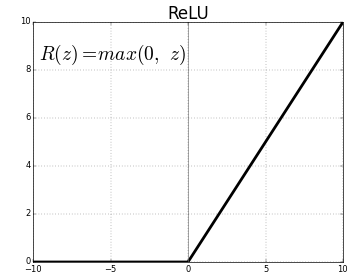
\includegraphics[width=8cm]{images/pruning/relu.png}
    \centering
    \caption{Rectified Linear Unit activation function}\label{fig:relu}
\end{figure}
    \item \textbf{Fully connected layer}: after several convolutional and max
        pooling layers, the high-level reasoning in the neural network is done
        via fully connected layers. Neurons in a fully connected layer have
        connections to all activations in the previous layer, as seen in
        non-convolutional artificial neural networks.
    \item \textbf{Loss layer}: it specifies how training penalizes the
        deviation between the predicted (output) and true labels and is
        normally the final layer of a neural network. Various loss functions
        appropriate for different tasks may be used. Softmax loss is used for
        predicting a single class of K mutually exclusive classes.
        Sigmoid cross-entropy loss is used for predicting K independent
        probability values in [0, 1]. Euclidean loss is used for regressing to
        real-valued labels.\cite{cnn}
\end{itemize}

\autoref{fig:channel_pruning} shows the channel pruning algorithm for a
single convolutional layer.
The aim is to reduce the number of channels of feature map B, while maintaining
outputs in feature map C.
Once the channels are pruned, corresponding channels of the filters that take
these channels as input can be removed. Moreover, filters that produce these
channels can be removed as well. It is clear that channel pruning involves
two key steps.

\begin{figure}[ht]
    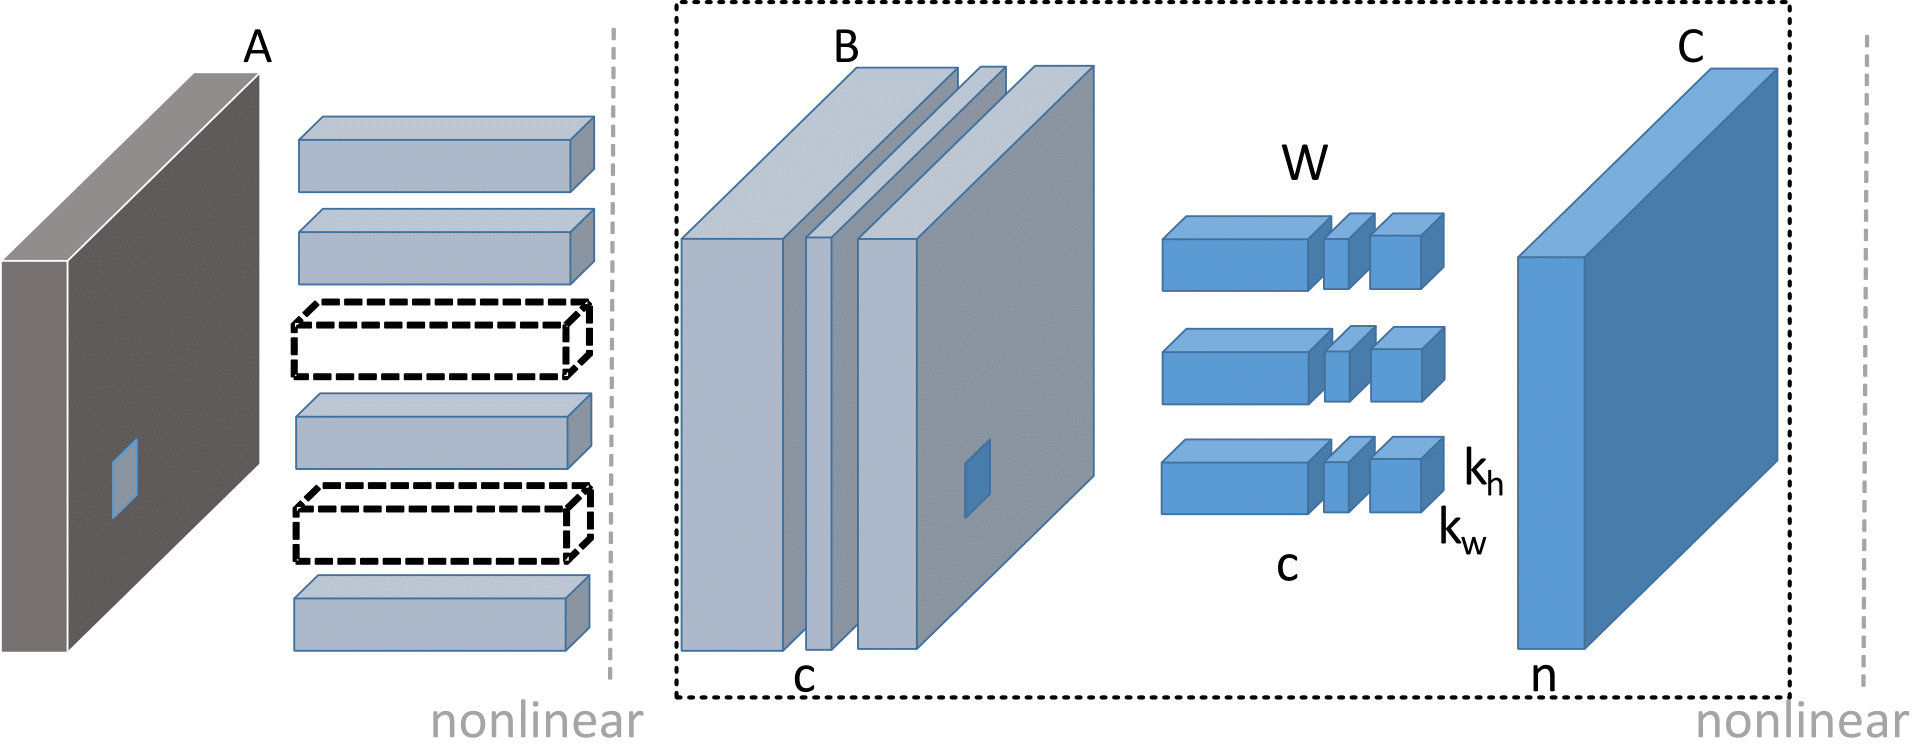
\includegraphics[width=8cm]{images/pruning/channel_pruning.png}
    \centering
    \caption{Channel Pruning for accelerating a CNN}\label{fig:channel_pruning}
\end{figure}

The first is the channel selection, since a proper channel combination to
maintain as much information needs to be selected.
The second is reconstruction. The following feature maps need to be
reconstructed using the selected channels. Motivated by this, the process is an
iterative two-step algorithm.

In the first step, the aim is to select most representative channels.
Since an exhaustive search is infeasible even for tiny networks, a LASSO
regression based method needs to be performed to figure out representative
channels and prune redundant ones.

In the second step, outputs are reconstructed with remaining channels with
linear least squares.

The whole model can be pruned applying the approach layer by layer
sequentially. For each layer, input volumes are obtained from the current input
feature map, and output volumes from the output feature map of the un-pruned
model.\cite{He_2017}

\subsubsection{Structured Pruning}
Pruning techniques can be broadly categorized as structured or unstructured.
Unstructured pruning does not follow a specific geometry or constraint. In most
cases, this technique needs extra information to represent sparse locations. It
depends on sparse representation for computational benefits. On the other hand,
structured sparsity places non-zero parameters at well-defined locations. This
kind of constraint enables modern CPUs and graphics processing units (GPUs) to
easily exploit computational savings.

\begin{figure}[ht]
    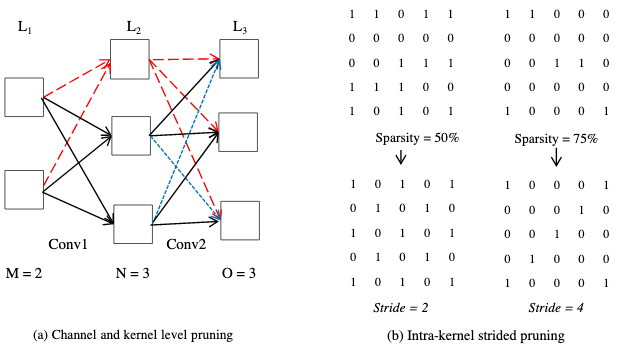
\includegraphics[width=\textwidth]{images/pruning/structured_pruning.png}
    \centering
    \caption{Structured Pruning}\label{fig:structured_pruning}
\end{figure}

Channel, kernel and intra-kernel sparsity could be a mean of structured
pruning. In channel level pruning, all the incoming and outgoing weights
to/from a feature map are pruned. Channel level pruning can directly produce a
lightweight network.
Kernel level pruning drops a full k × k kernel, whereas the intra-kernel
sparsity prunes weights in a kernel. The intra kernel strided sparsity can
significantly speed-up convolution layer processing.
The kernel level pruning is a special case of intra-kernel sparsity with
100\% pruning. These granularities can be applied in various combinations and
different orders.\cite{Anwar_2017}

\subsection{Pruning pipeline}
Training, pruning, fine-tuning
1506.02626 \- Learning both Weights and Connections for Efficient Neural Networks
\lipsum[1]

\subsection{Practical examples with Pruning}
\lipsum[1]

\subsection{Sparsity-accuracy trade-offs}\label{subsec:tradeoff}
\lipsum[1]

\section{Per-Layer Pruning Configuration With Heuristic}\label{sec:heuristic}
\lipsum[1]

\subsection{What's a heuristic?}
\lipsum[1]

\subsection{Heuristic details}
Explain in details the technique and the reasons behind
\lipsum[1]

\subsection{Custom heuristic formula}
\lipsum[1]
